\subsection{Solving Ordinary differential equations}
In this part consider the arbitrary ODE:
\begin{equation}
	\label{eq:ode}
	\begin{multlined}
		\mathcal{D}\left (x, y, y^{(1)}, \dots, y^{(n)}\right) = 0, \quad x \in \Omega = [0, 1] \subset  R \\
		B(y) = 0, \quad x \in \partial \Omega = \{0, 1\}
	\end{multlined}
\end{equation}
, where $\mathcal{D}(\dots)$ - differential operator, $B(y)$ - boundary conditions function. 
\begin{equation*}
	B(y) = \begin{cases}
		D(y) = 0, \quad x \in \partial \Omega_D = \{0, 1\} \\
		N(y) = 0, \quad x \in \partial \Omega_N = \{0, 1\} 
	\end{cases}, \partial \Omega_N \cup \partial \Omega_D = \partial \Omega
\end{equation*}
where $D(y)$ - Dirichlet boundary conditions and $\partial \Omega_D$ boundary for these conditions, N(y) - Neumann boundary conditions and $\partial \Omega_N$ is bound them.
All of the equations considered now and in the future in this work will be defined as \eqref{eq:ode}.

For solving this equation will be considered two methods, weighted residuals method \cite{fletcher2012computational} (Bubnov-Galerkin) and finite differences method \cite{dimov2019finite}.

For concreteness, ODE example for consideration:
\begin{equation*}
	\begin{multlined}
		\dfrac{d}{d x^2} y(x) + 2y = sin(2x) \left ( 1 - 2 sin(2x) \right), x \in [0, 1]\\
		y(0) = 0, \quad \dfrac{d}{dx} y \Big|_{x = 0} = 1
	\end{multlined}
\end{equation*}
, where $y = \dfrac{1}{2} sin(2x)$ - analytical solution.

\subsubsection{Galerkin method}
The key idea is to define the solution as:
\begin{equation}
	\label{eq:galerkin_presentation}
	y_h = \phi_0 + \sum_{i = 1}^N a_i \phi_i(x)
\end{equation}
and $\phi_0$ satisfy all boundary conditions $\phi_0: B(\phi_0) = 0 \implies \phi_0(0) = 0, \phi_0(1) = 1$ and $\phi_i$ satisfy the homogenous boundary conditions $\phi_i(0) = \phi_i(1) = 0$. The solution to the problem is a some weighted sum of linearly independent functions that satisfy the boundary conditions and in the general case satisfy the initial conditions too. For calculation, the coefficients use minimization residual method, where:
\begin{equation*}
	\min_{a_1, \dots, a_n} R(a_1, \dots, a_n) = \int_{\Omega} \mathcal{D}(y_h) d\Omega + \int_{\partial \Omega_N} N(y_h) d\partial \Omega
\end{equation*}
From \cite{fletcher2012computational} is known that $R$ does not equal zero in the general case and for evaluating the coefficients use the integration with weight function:
\begin{equation*}
	\int_{\Omega} w R(a_1, \dots, a_n) d\Omega = \int_{\Omega} w \mathcal{D}(y_h) d\Omega + \int_{\partial \Omega_N} w N(y_h) d\partial \Omega = 0
\end{equation*}
, where $w = \psi_i$, weight functions. The residual and weight functions must be orthogonal.
In a more general case without using $phi_0$ the residual is:
\begin{equation*} 
	\begin{multlined}
		\int_{\Omega} \psi_j R(a_1, \dots, a_n) d\Omega = \int_{\Omega} \psi_i \mathcal{D} \left ( \sum_{i = 1}^N a_i \phi_i(x) \right ) d\Omega + \int_{\partial \Omega} \psi_j B \left ( \sum_{i = 1}^N a_i \phi_i(x) \right ) d\partial \Omega = \\ =
		\int_{\Omega} \psi_j \mathcal{D} \left ( \sum_{i = 1}^N a_i \phi_i(x) \right ) d\Omega + \int_{\partial \Omega} \psi_j B \left ( \sum_{i = 1}^N a_i \phi_i(x) \right ) d\partial \Omega = \text{ if $\mathcal{D}, \mathcal{B}$ are linear operators } = \\ = \int_{\Omega} \sum_{i = 1}^N  a_i \psi_j \mathcal{D}(\phi_i(x)) d\Omega + \int_{\partial \Omega} \sum_{i = 1}^N  a_i \psi_j B(\phi_i(x)) d\partial \Omega = 0
	\end{multlined}
\end{equation*}
From the equation above system of algebraic equations can be constructed and solve it for unknown coefficients $a_i$.
\subsubsection{Galerkin method, special case}
If $w$ is delta Dirac function, then the Galerkin method also called the Pointwise collocation method, which more easy for implementation.
\begin{equation}
	\begin{multlined}
		w = \delta(x - x_k), x_k \in X \subset \Omega, \text{ and } \| X \| = K, \\
		\int_{\Omega} \delta(x - x_k) R(a_1, \dots, a_n) d\Omega = \int_{\Omega} \delta(x - x_k) \mathcal{D} \left ( \sum_{i = 1}^N a_i \phi_i(x) \right ) d\Omega + \\ + \int_{\partial \Omega} \delta(x - x_k) B \left ( \sum_{i = 1}^N a_i \phi_i(x) \right ) d\partial \Omega
		 = \mathcal{D} \left ( \sum_{i = 1}^N a_i \phi_i(x_k) \right ) + B \left (\sum_{i = 1}^N a_i \phi_i(x_k) \right )
	\end{multlined}
\end{equation}
In case when the number of points of collocation more then the number of unknown coefficients the problem solves via optimization techniques, the least-squares method for example.

\subsubsection{Finite difference method}
First of all, the finite difference derivative is:
\begin{itemize}
	\item Left derivative \begin{equation}
		\label{eq:left_der}
		\dfrac{d y}{d x} \Big|_{x = x_i} = \dfrac{y(x_i) - y(x_{i - 1})}{x_i - x_{i - 1}}
	\end{equation}
	\item Central derivative \begin{equation}
		\label{eq:central_der}
		\dfrac{d y}{d x} \Big|_{x = x_i} = \dfrac{y(x_{i + 1}) - y(x_{i - 1})}{x_{i + 1} - x_{i - 1}}
	\end{equation}
	\item Right derivative \begin{equation}
		\label{eq:right_der}
		\dfrac{d y}{d x} \Big|_{x = x_i} = \dfrac{y(x_{i + 1}) - y(x_i)}{x_{i + 1} - x_i}
	\end{equation}
\end{itemize}
Actually, the approximation quality better for the central difference derivative. The derivatives of higher order can be constructed from the first-order derivatives (left, right, central). For example:
\begin{equation*}
	\dfrac{d^2 y}{d x^2} \Big|_{x = x_i} = \dfrac{d}{d x} \Big|_{x = x_i} \left [ \dfrac{y(x_{i + 1})}{x_{i + 1} - x_i} \right ] - \dfrac{d}{d x} \Big|_{x = x_i} \left [ \dfrac{y(x_{i - 1})}{x_i - x_{i - 1}} \right ] = \dfrac{y(x_{i + 1}) - y(x_i)}{x_{i + 1} - x_i} - \dfrac{y(x_i) - y(x_{i - 1})}{x_i - x_{i - 1}}
\end{equation*}
When the grid uniformly distributes the $x_i$ values: $x_{i + 1} - x_i = d$:
\begin{equation*}
	\dfrac{d^2 y}{d x^2} \Big|_{x = x_i} = \dfrac{y(x_{i + 1}) - 2 y(x_i) + y(x_{i - 1})}{d^2}
\end{equation*}
So, the idea of the FDM is to substitute the finite derivatives and solve algebraic equations. 
\begin{equation*}
	\mathcal{D} (x, y, y^{(1)}, \dots, y^{(n)}) \Big|_{x = x_i} = \mathcal{D} \left ( x_i, y(x_i), \dfrac{y(x_{i + 1}) - y(x_{i - 1})}{x_{i + 1} - x_{i - 1}}, \dots, \dfrac{y(x_{i + n - 1}) + \dots + y(x_{i - n + 1})}{d^n} \right )
\end{equation*}
And the same way for the boundary conditions:
\begin{equation*}
	B(y) \Big|_{x = x_i}  = \begin{cases}
		D(y) = 0, \quad x \in \partial \Omega_D = \{0, 1\} \\
		N(y) = 0, \quad x \in \partial \Omega_N = \{0, 1\} 
	\end{cases} 
\end{equation*}
After the solving equations, the values of $y_i$ are known and needed to be interpolated over the domain $\Omega$.
\subsubsection{Comparison of the provided methods}	
Methods are very different, the FDM provides the solution in the fixed nodes and interpolates the solution from these nodes overall domain, on the other hand, the Galerkin method provides approximation solution in the mean sense over the domain. This difference makes the variability of the interpolation methods or basis functions for calibration of the numerical solution quality. The strong and ill sides of the FDM are high quality of the solution over the nodes, but the interpolation process leads to the Runge phenomenon, besides the size of the grid has a tremendous influence on the solution quality. 
The Galerkin method provides the approximation over the domain and strongly depends on the initial choice basis functions, so, there is the probability, that solution has a compact form.

It will be good if the strong sides of these methods will be combined into one approximator. Ideal case, when the number of terms increases, the solution quality increase too.

First of all, using the theorem \ref{sigmoidal_expansion} and the solution form \eqref{eq:galerkin_presentation}:
\begin{equation}
	\label{eq:perceptron_ode}
	y_h(x) = \phi_0(x) + \sum_{i = 1}^K \alpha_i \sigma(\beta_i x + \gamma_i)
\end{equation}
$\phi_0$ also satisfy the boundary conditions. 
For this solution from the theorem known, that the approximation quality strongly depends on the number of terms in the series, in addition, this form satisfies the boundary conditions, as in the Galerkin method. Now, the quality of the solution is guaranteed by the theorem and the question about basis function is solved. Moreover, using points collocation method:
\begin{equation}
	\label{eq:loss_galrekin}
	\begin{multlined}
		\mathcal{L} = \dfrac{1}{| X |} \sum_{x \in X} \left [ \| R(x; p_1, 
		\dots, p_N) \|^2 \right ], \quad X \in \Omega \subset R, p_i = (\alpha_i, \beta_i, \gamma_i) \in P \subset R^3 \\
		\textbf{Coefficients :} \min_{p_i} \mathcal{L} = \begin{cases}
			\dfrac{\partial \mathcal{L}}{\partial \alpha_i} = 0 \\[10pt]
			\dfrac{\partial \mathcal{L}}{\partial \beta_i} = 0 \\[10pt]
			\dfrac{\partial \mathcal{L}}{\partial \gamma_i} = 0
		\end{cases}
	\end{multlined}
\end{equation}
Currently, the solution is found using the least-squares method, which leads to solving the system of equations with not one solution. For each solution, the loss function should be calculated and chose the parameter where problem has a minimum value.

For this approach calculation of the derivatives for a differential operator should be provided:
\begin{equation}
	\label{eq:bad_system}
	\begin{multlined}
		\dfrac{d y_h}{d x} = \dfrac{d}{d x} \left [ \phi_0(x) + \sum_{i = 1}^K \alpha_i \sigma(\beta_i x + \gamma_i) \right ] = \dfrac{d}{d x} \phi_0(x) + \sum_{i = 1}^K \alpha_i \dfrac{d}{d x} \sigma(\beta_i x + \gamma_i) = \\ = \dfrac{d}{d x} \phi_0(x) + \sum_{i = 1}^K \alpha_i \beta_i  \sigma(\beta_i x + \gamma_i) (1 - \sigma(\beta_i x + \gamma_i))
	\end{multlined}
\end{equation}
The form of the derivative immediately told that the solving of equations \eqref{eq:bad_system} is very unstable and there are a lot of roots. On the other hand, using the numerical derivative \eqref{eq:left_der}, \eqref{eq:central_der}, \eqref{eq:right_der} leads to:
\begin{equation}
	\label{eq:good_system}
	\begin{multlined}
		\dfrac{d y_h}{d x} \Big|_{x = x_i} \approx \dfrac{y_h(x_{i + 1}) - y_h(x_{i - 1})}{2d} = \dfrac{1}{2d} \left [ y_h(x_{i + 1}) - y_h(x_{i - 1}) \right ]
	\end{multlined}
\end{equation}

\subsubsection{Artificial neural networks (ANN)}	
Definition from Wikipedia is ``Artificial neural networks (ANN) or connectionist systems are computing systems vaguely inspired by the biological neural networks that constitute animal brains. Such systems "learn" to perform tasks by considering examples, generally without being programmed with task-specific rules``, or the second one definition: ``A mathematical model, as well as its software or hardware implementation, built on the principle of organization and functioning of biological neural networks - networks of nerve cells of a living organism.''
\begin{figure}[h]
	\centering
	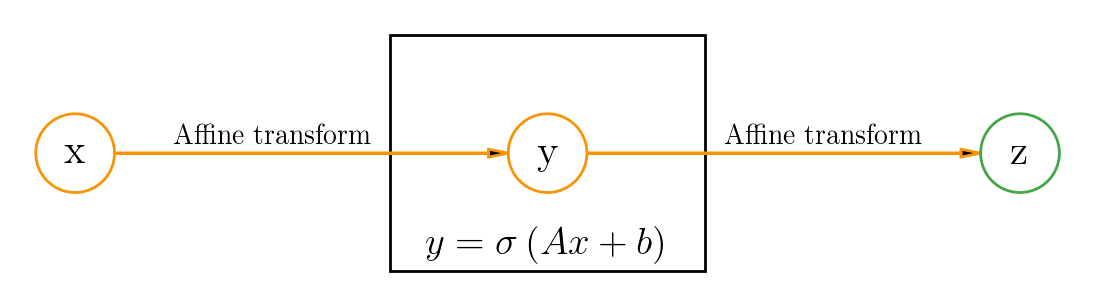
\includegraphics[width=1 \textwidth]{images/chapter2/simple_net.png}
	\caption{The illustration of \eqref{eq:perceptron_ode}. One layered neural network}
	\label{fig:simple_net}
\end{figure}


These definitions are similar, in the sense that the input signal passes through the set of ordered simple operations or layers, and at the end of these operations the output is the result of the neural network. The order of these operations also called the architecture of the neural network. There are a lot of different types of layers\footnote{The zoo of neural network types: \href{https://www.asimovinstitute.org/neural-network-zoo/}{ANN zoo}}, the most widely used is the fully connected layer or dense layer as in figure \ref{fig:simple_net}.
Looking more precisely the neural network is sequence of affine transformations (edges) and nonlinear transformation (nodes):
\begin{equation*}
	\begin{multlined}
		\mathcal{N}(x) = \left [ A^2 \circ \phi^1 \circ A^1 \right ] (x) = A^2 \phi^1 \left (A^1 x + b^1 \right ) + b^2 \\ A^1 \in R^{m \times n}, A^2 \in R^{k \times m}, b^1 \in R^m, b^2 \in R^k, x \in R^n
	\end{multlined}
\end{equation*}
In general case $l$ layered neural network is:
\begin{equation}
	\label{eq:neural_net}
	\mathcal{N} = A^l \circ \phi^{l - 1} \circ A^{l - 1} \circ \dots \circ \phi^1 \circ A^1 = A^l \left [ \phi^{l - 1} \left [ \dots \left [ A^1 (x) + b^1 \right ] \dots \right ] + b^{l - 1} \right] + b^l
\end{equation}
where $A^i, \forall i \in \{1, \dots, l\}$ is the parameter that must be found. For the successful using the neural networks:
\begin{itemize}
	\item Define the architecture
	\item Define the loss function
	\item Choose a suitable optimization algorithm \begin{itemize}
		\item How the optimization process looks
		\item Existing optimization algorithms
	\end{itemize}
\end{itemize}

\subsubsection{Optimization part. Backpropagation algorithm}

The main goal is getting the numerical solution of the DE and for this aim is to use the residual \eqref{eq:loss_galrekin} and minimize it over the parameters of the neural network:
\begin{equation*}
	\min_{A^l, b^l, \dots, A^1, b^1} \mathcal{L} = \min_{A^l, b^l, \dots, A^1, b^1} \mathcal{L} = \dfrac{1}{| X |} \sum_{x \in X} \| R(x) \|^2
\end{equation*}
Now, how to minimize this complex function? Using the least-squares leads to solving the equations or use gradient-based optimization. For the estimation, the values of the neural network parameters use the gradient-based methods and iteratively goes to the local minimum(!). Suppose, the for the point collocation method randomly choose the set of points at the $k$-th step, the loss is calculated and gradients are calculated:.
\begin{equation}
	\nabla A_k^l = \nabla_{A^l} \mathcal{L}_k, \quad A_{k + 1}^l = A_k^l - \lambda(k) \psi(\nabla A_k^l)
\end{equation}
the $\psi$ is the main part of the particular algorithm because using the $\psi(x) = x$, stochastic gradient descent (SGD) immediately have gotten. Using different $\psi$, the corresponding methods are obtained \cite{Adadelta}, \cite{Adagrad}, \cite{Adam}, \cite{Diffgrad}.
\paragraph{Optimizers comparison}
To demonstrate the quality of various optimization algorithms, a simple neural network architecture was chosen and trained to approximate the function. Lines are the average value of the loss function at a particular iteration, the region of the corresponding color is the region in which the error may lie on average. To collect such statistics, the neural network was trained by each optimizer 25 times.
The results are presented in the figure \ref{fig:optimizers}.
\begin{figure}[h]
	\centering
	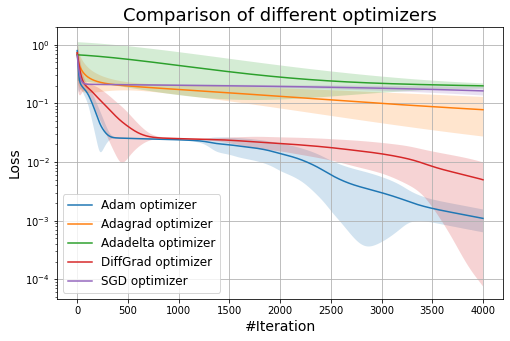
\includegraphics[width=0.75 \textwidth]{images/chapter2/optimizers.png}
	\caption{Comparison of different optimizers for fixed neural network architecture}
	\label{fig:optimizers}
\end{figure}

Consider the sequence of the operators \eqref{eq:neural_net} and the quality function or loss function $\mathcal{L}$. Currently not important what loss function and the nature of the operators:
\begin{equation*}
	\begin{multlined}
		\mathcal{N} = A^l \circ \phi^{l - 1} \circ A^{l - 1} \circ \dots \circ \phi^1 \circ A^1, \quad \mathcal{L} = \mathcal{L} \left ( \mathcal{N} \right )
	\end{multlined}
\end{equation*}
For efficient evaluating the gradients over the parameters exists a backpropagation\footnote{
	In machine learning, backpropagation (backprop, BP) is a widely used algorithm in training feedforward neural networks for supervised learning. Generalizations of backpropagation exist for other artificial neural networks (ANNs), and for functions generally – a class of algorithms referred to generically as "backpropagation" - from Wikipedia
} algorithm \cite{chauvin2013backpropagation}. The key idea is to use the chain rule for the derivative:
\begin{equation*}
	\begin{cases}
		\dfrac{\partial \mathcal{L}}{\partial A^l} = \nabla_{A^l}\mathcal{L} \\[10pt]
		\dfrac{\partial \mathcal{L}}{\partial A^{l - 1}} = \left [ \phi^l \right ]^{'} \left [ A^{l - 1} \right ]^T \nabla_{A^l}\mathcal{L} \\[10pt]
		\dfrac{\partial \mathcal{L}}{\partial A^{l - 2}} = \left [ \phi^{l - 1} \right ]^{'} \left [ A^{l - 2} \right ]^T  \left [ \phi^l \right ]^{'} \left [ A^{l - 1} \right ]^T \nabla_{A^l}\mathcal{L} =  \left [ \phi^{l - 1} \right ]^{'} \left [ A^{l - 2} \right ]^T  \dfrac{\partial \mathcal{L}}{\partial A^{l - 1}} \\[10pt] 
		\text{For k-th derivative in the same way:} \\[10pt]
		\dfrac{\partial \mathcal{L}}{\partial A^{l - k}} = \left [ \phi^{l - k + 1} \right ]^{'} \left [ A^{l - k} \right ]^T  \dfrac{\partial \mathcal{L}}{\partial A^{l - k + 1}}
	\end{cases} 
\end{equation*}
Now it is known how a neural network works, how it is trained and why a solution can be built with arbitrary accuracy. Next, we will consider different architectures of neural networks for solving different problems, and different approaches, for example, the approach based on the Galerkin method, when the Dirichlet boundary conditions are embedded in a neural network. There is also an approach based on the Ritz method that reduces the solution of the equation to an extremal problem. For example, when solving equations, it is possible to integrate the boundary conditions into the approximator structure \cite{Lagaris_1998} \cite{liu2019solving}.
Here the solution is presented in the form:
\begin{equation}
	\label{eq:simple_solver}
	y_h = A(x) + B(x) \mathcal{N}(x)
\end{equation}
where $A$ satisfies the boundary conditions of the first and second kind, where $A$ satisfies the boundary conditions of the first and second kind, and $B$ is in a sense a function of distance, or rather a function that “removes” the values of the model (neural network) at the boundary. 
\paragraph{Example}
Consider equation $\phi \left ( x, y, \dfrac{d y}{d x}, \dfrac{d^2 y}{d x^2} \right ) = 0$ and boundary conditions $y(0) = y_0, y(1) = y_1$. In this case, the solution will be built in the form:
\begin{equation*}
	y_h = (1 - x) y_0 + x y_1 + (1 - x) x \mathcal{N}(x)
\end{equation*}
Thus, for such a form, a neural network is only part of the solution, for points within a region. It is clear that the name of the complex boundary conditions for the partial differential equation to construct a solution in this form is very difficult. In this form, it is convenient to search for a solution having homogeneous boundary conditions of the first kind. You can use the results from \cite{fletcher2012computational}, where it is proposed to construct the solution in such a way as to satisfy only conditions of the first kind, and transfer conditions of the second and third kind to the neural network again (to the loss function), example:
\begin{equation*}
	\begin{multlined}
		\phi \left ( x, y, \dfrac{d y}{d x}, \dfrac{d^2 y}{d x^2} \right ) = 0, \quad y(0) =  y_0, \dfrac{d y}{d x} \Big|_{x = 0} = y_1 \\
		y_h = (1 - x) y_0 + B(x) \mathcal{N}(x), \quad \mathcal{L}^{'} = \mathcal{L} + \lambda \left \| \dfrac{d y_h}{d x}\Big|_{x = 0} - y_1  \right \|
	\end{multlined}
\end{equation*}
Another approach \cite{cao2016locally} also embeds the boundary conditions in the general solution, however, it occurs due to an additional term that estimates the error between the conditions and the solution itself at the boundary and embeds the additional term in a row in order to satisfy the conditions. In fact, every few iterations of the network training, the term is recalculated (a small system of equations is solved) and adjusted to the boundary conditions. Not quite an easy way to implement, however, the quality of the final solution depends on the boundary conditions, on the structure of the additional unit and the necessary accuracy. Models based on the Galerkin method are quite common, so the authors \cite{Sirignano_2018} proposed the structure of the model so that, with an increase in the dimension of the problem, the quality of the solution remains acceptable. Their model looks interesting, combines many breakthrough deep learning approaches, but in view of this, the speed of learning is very low. The authors themselves in their work provide an assessment of the training time and the necessary capacities for this - it takes an order of magnitude more time on a conventional personal computer than classical approaches require, but the main goal is high-dimensional tasks, where the algorithm really showed good quality. All approaches proposed and considered below can be divided into 2 groups: 
\begin{itemize}
	\item Embed in the solution itself \cite{Lagaris_1998} \cite{liu2019solving} \cite{cao2016locally}
	\item Consider a conditional problem solved by the Lagrange method. In the learning process, the model learns not only to solve the equation itself, but is also fined for not satisfying the boundary conditions \cite{Pun_2019}
\end{itemize}
Each group has its own characteristics, so for methods from the first group, the high quality of the solution is characteristic, but the difficulty of drawing up the presentation of the solution is high. The second group is characterized by a not very high quality solution, especially at the borders, however, with sufficient training time and properly selected regularization, this problem is solved, but the plus is the ease of implementation.

\subsubsection{Examples of ODE}
\begin{equation*}
	\dfrac{d y}{d x} = sin(x), \quad y(0) = -1
\end{equation*}

\begin{tabular}{c c c}
 Method & Parameters num & Accuracy \\
 FDM & 10  & $7.82 10^{-3}$  \\
 FDM & 25  & $2.88 10^{-3}$  \\
 FDM & 50  & $1.44 10^{-3}$  \\
 FDM & 100  & $0.69 10^{-3}$ \\
  FDM & 200  & $0.34 10^{-3}$ \\
 ANN & 8  & $0.298 10^{-3}$  \\
 ANN & 10  & $0.111 10^{-3}$ \\
 ANN & 20  & $0.0105 10^{-3}$  \\
ANN & 50  & $0.00413 10^{-3}$
\end{tabular}